\chapter{Simulation}
Before actually building the system and experimenting on an expensive quadcopter in real world environment,
it is cheaper, safer and easier to do tests in a simulated environment. 

The PX4 Firmware repository\cite{PX4Repository} contains Gazebo simulation files to give developers a head 
start in simulation of their product. Upon these simulation quadcopter models LIDAR sensors can be placed and 
moved around with ease, without the need of wiring or external infrastructure. This simulation is 
suitable for Software in the loop (SITL) testing, meaning that the same software developed for the simulation
can be used on a real quadcopter.



\section{Robot Operating System}
Robot Operating system (ROS) is a set of software libraries and tools that help developers to build robust 
general-purpose robot applications\cite{ROSWebsite}. ROS provides hardware abstraction of the underlying 
robot, generalizes the interfacing of these robots and allows simple high-level usage.


The core component of ROS is a public-subscribe communication protocol similar to MQTT protocol
used on the field of IoT. The ROS system is comprised of a number of independent communicating parties called 
nodes. Each node can subscribe to multiple topics and receive a stream of messages published to these topics 
by other nodes. For example a temperature filter node might subscribe to a topic of "/temperature\_sensor" 
and publish the filtered temperature values to a topic called "/filtered\_temperature\_sensor". 
The benefit using this solution is that the nodes achieve communication exclusively via this protocol 
so each node lives independently from another. Nodes in ROS do not need to be on the same system or 
even on the same architecture. Nodes can be run on different computers or even on microcontrollers or 
smartphones making the system flexible.

\begin{figure}[!ht]
    \centering
    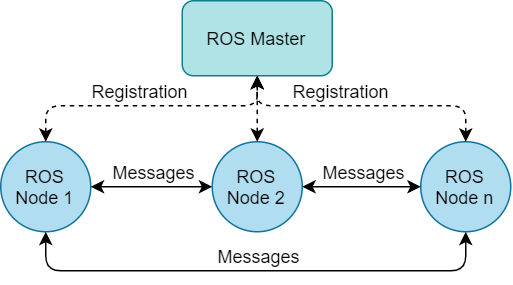
\includegraphics[width=100mm, keepaspectratio]{figures/ros_pubsub.png}
    \caption{ROS publish subscribe communication}
    \label{fig:ros_pubsub}
\end{figure}

To start a ROS session, a ROS Master needs to be started first. After starting the master, nodes can be 
started and each one registers the topics it wants to subscribe/publish to. The master handles these requests
and helps the nodes to establish connection between each other so communication can be started. 

ROS is language independent so nodes can be implemented in different programming languages. While C++ is 
the most common language for product development, official Python wrappers can be used for fast 
prototyping.


\section{Gazebo Simulator}
Gazebo\cite{GazeboWebsite} is an open-source 3D simulator for robotics, with the ability to accurately simulate robots in complex
indoor or outdoor environments. It is similar to game engines, but produces more realistic, physically correct
behavior. Gazebo is free, open-source, actively developed and has gained high popularity during the last years. 

Gazebo comes with a growing number of robots and sensors. For simulations one can choose from the officially 
available robots or create a custom robot using SDF files. Any of these robots can be customized and any 
number of sensors can be added. Using simulations sensor data can be generated and development can be started 
without having the actual hardware.

\begin{figure}[h]
    \centering
    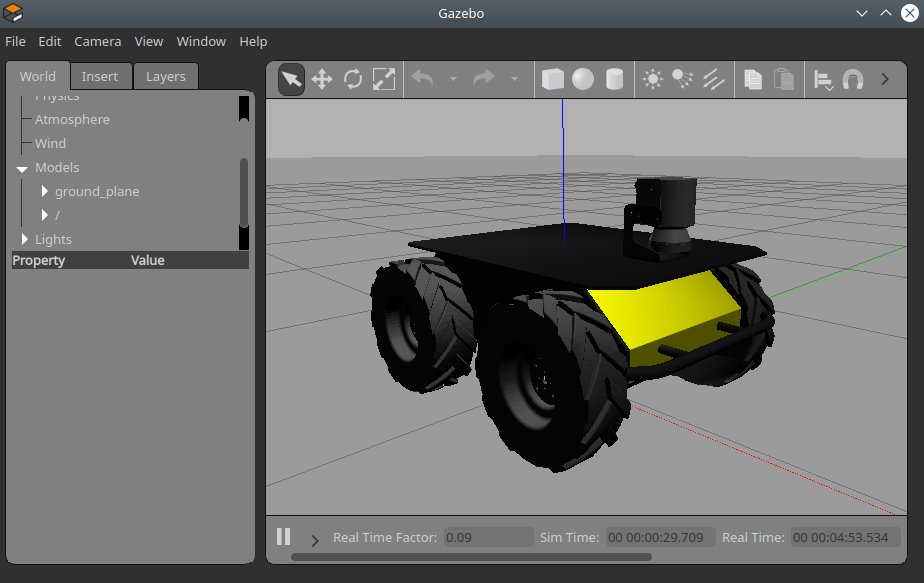
\includegraphics[width=100mm, keepaspectratio]{figures/husky.png}
    \caption{Gazebo ROS Husky robot demo}
    \label{fig:ros_husky}
\end{figure}

Why Gazebo is particularly interesting, is because it can be started in a ROS compatible mode. Gazebo
started with ROS wrapper will actively channel all sensor readings, states and many more to ROS topics, 
allowing nodes outside of the simulation to subscribe and publish to these topics. Using this technique nodes 
can be developed in a truly hardware independent manner. The simulation can be replaced by a real robot
and the nodes developed during this phase can be used without changes on the real hardware. For example a 
Husky robot can be simulated in Gazebo and controlled through ROS. The Gazebo simulation of a Husky 
can be seen on figure \ref{fig:ros_husky}.


\section{PX4 Autopilot Software}
PX4 is a powerful open-source autopilot flight stack. PX4 can control many different vehicle frames and vehicle 
types, supports wide variety of sensors and peripherals. The project is a part of Dronecode, a nonprofit
foundation working on open-source projects to achieve standardization of drones.\cite{PX4Website} 

The core component of PX4 is the flight stack or flight controller that controls the motors based on sensor
measurements and executes commands received from ground control. Besides the flight stack the repository 
also contains Gazebo simulation files of multiple vehicles and an extensive \verb|Makefile| that makes 
starting simulations relatively easy. 

\subsection{PX4 simulation using MAVROS}
The logical units of the simulation can be seen on figure \ref{fig:px4_sitl_simulation}.
By executing a \verb|make| command the Gazebo Simulator, the PX4 SITL flight stack and the API/Offboard units
are started at once. The PX4 SITL flight stack connects on a TCP port to the simulator, receives sensor data, 
calculates and sends motor and actuator values to the simulated vehicle. There are two options for the navigation
of the simulated drone: using an Offboard API or a Ground Control Station. For autonomous flight control an 
Offboard API needs to be used and MAVROS is a suitable choice, it basically offers a ROS interface for 
the drone. It forwards all messages from the flight stack to ROS topics and vice versa.

\begin{figure}[h]
    \centering
    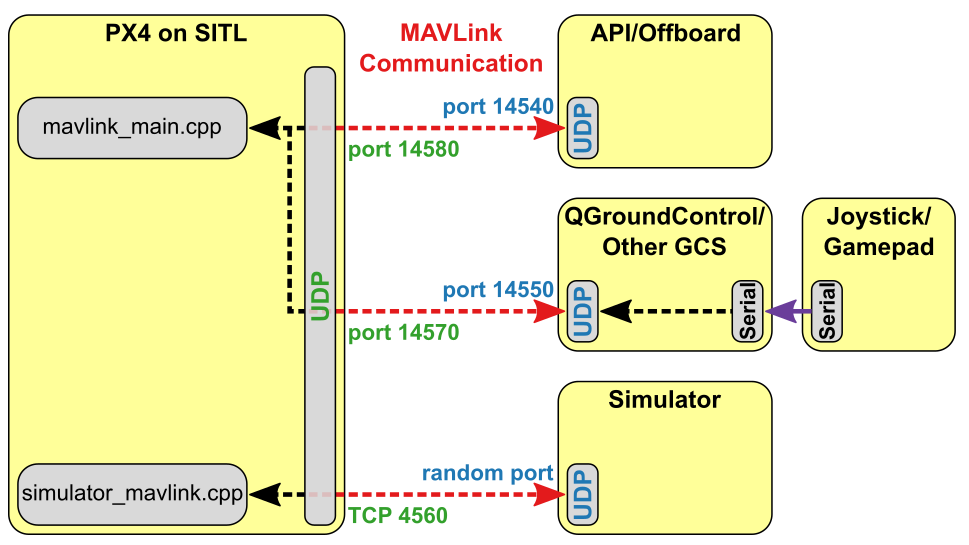
\includegraphics[width=120mm, keepaspectratio]{figures/px4_sitl_overview.png}
    \caption{PX4 SITL Simulation Outline \cite{PX4Simulation}}
    \label{fig:px4_sitl_simulation}
\end{figure}

\subsection{PX4 simulation using Gazebo with ROS wrapper}

%New sensors from simulator through SITL or straight to ROS
Drone models are described using SDF files that are XML based and by modifying these files new sensors can 
be added. Gazebo loads the selected vehicle and the sensors, but if a selected sensor is not supported by
PX4, its measurements will not be forwarded to MAVROS and therefore to ROS topics. It can be troublesome 
to always use sensors that are supported by the flight controller, not to mention that the MAVLink protocol 
is designed for small messages so the bandwidth can be too low in some cases. Luckily Gazebo can 
be started with a ROS wrapper and therefore all sensors can be accessed on ROS topics. However this technique
cannot be used on a real drone with the original PX4 firmware, because it purely relies on MAVLink messages, 
but for simulation purposes it's an elegant solution. This modified overview of the units used for simulation
and a screenshot of an Iris drone simulated in Gazebo can be seen on figure \ref{fig:px4_sitl_ros_wrapper}. 
MAVROS is still needed to be run, because there are some messages that would not be published to ROS otherwise.

\begin{figure}[h]
    \centering
    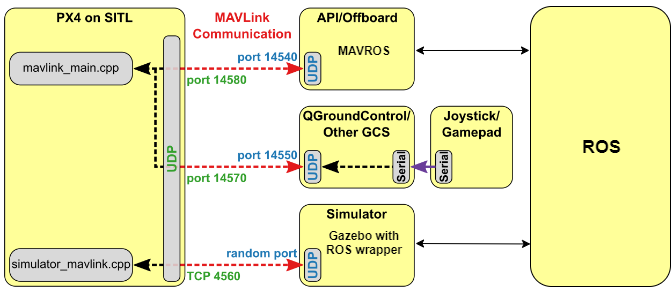
\includegraphics[width=140mm, keepaspectratio]{figures/px4_sitl_with_ros.png}
    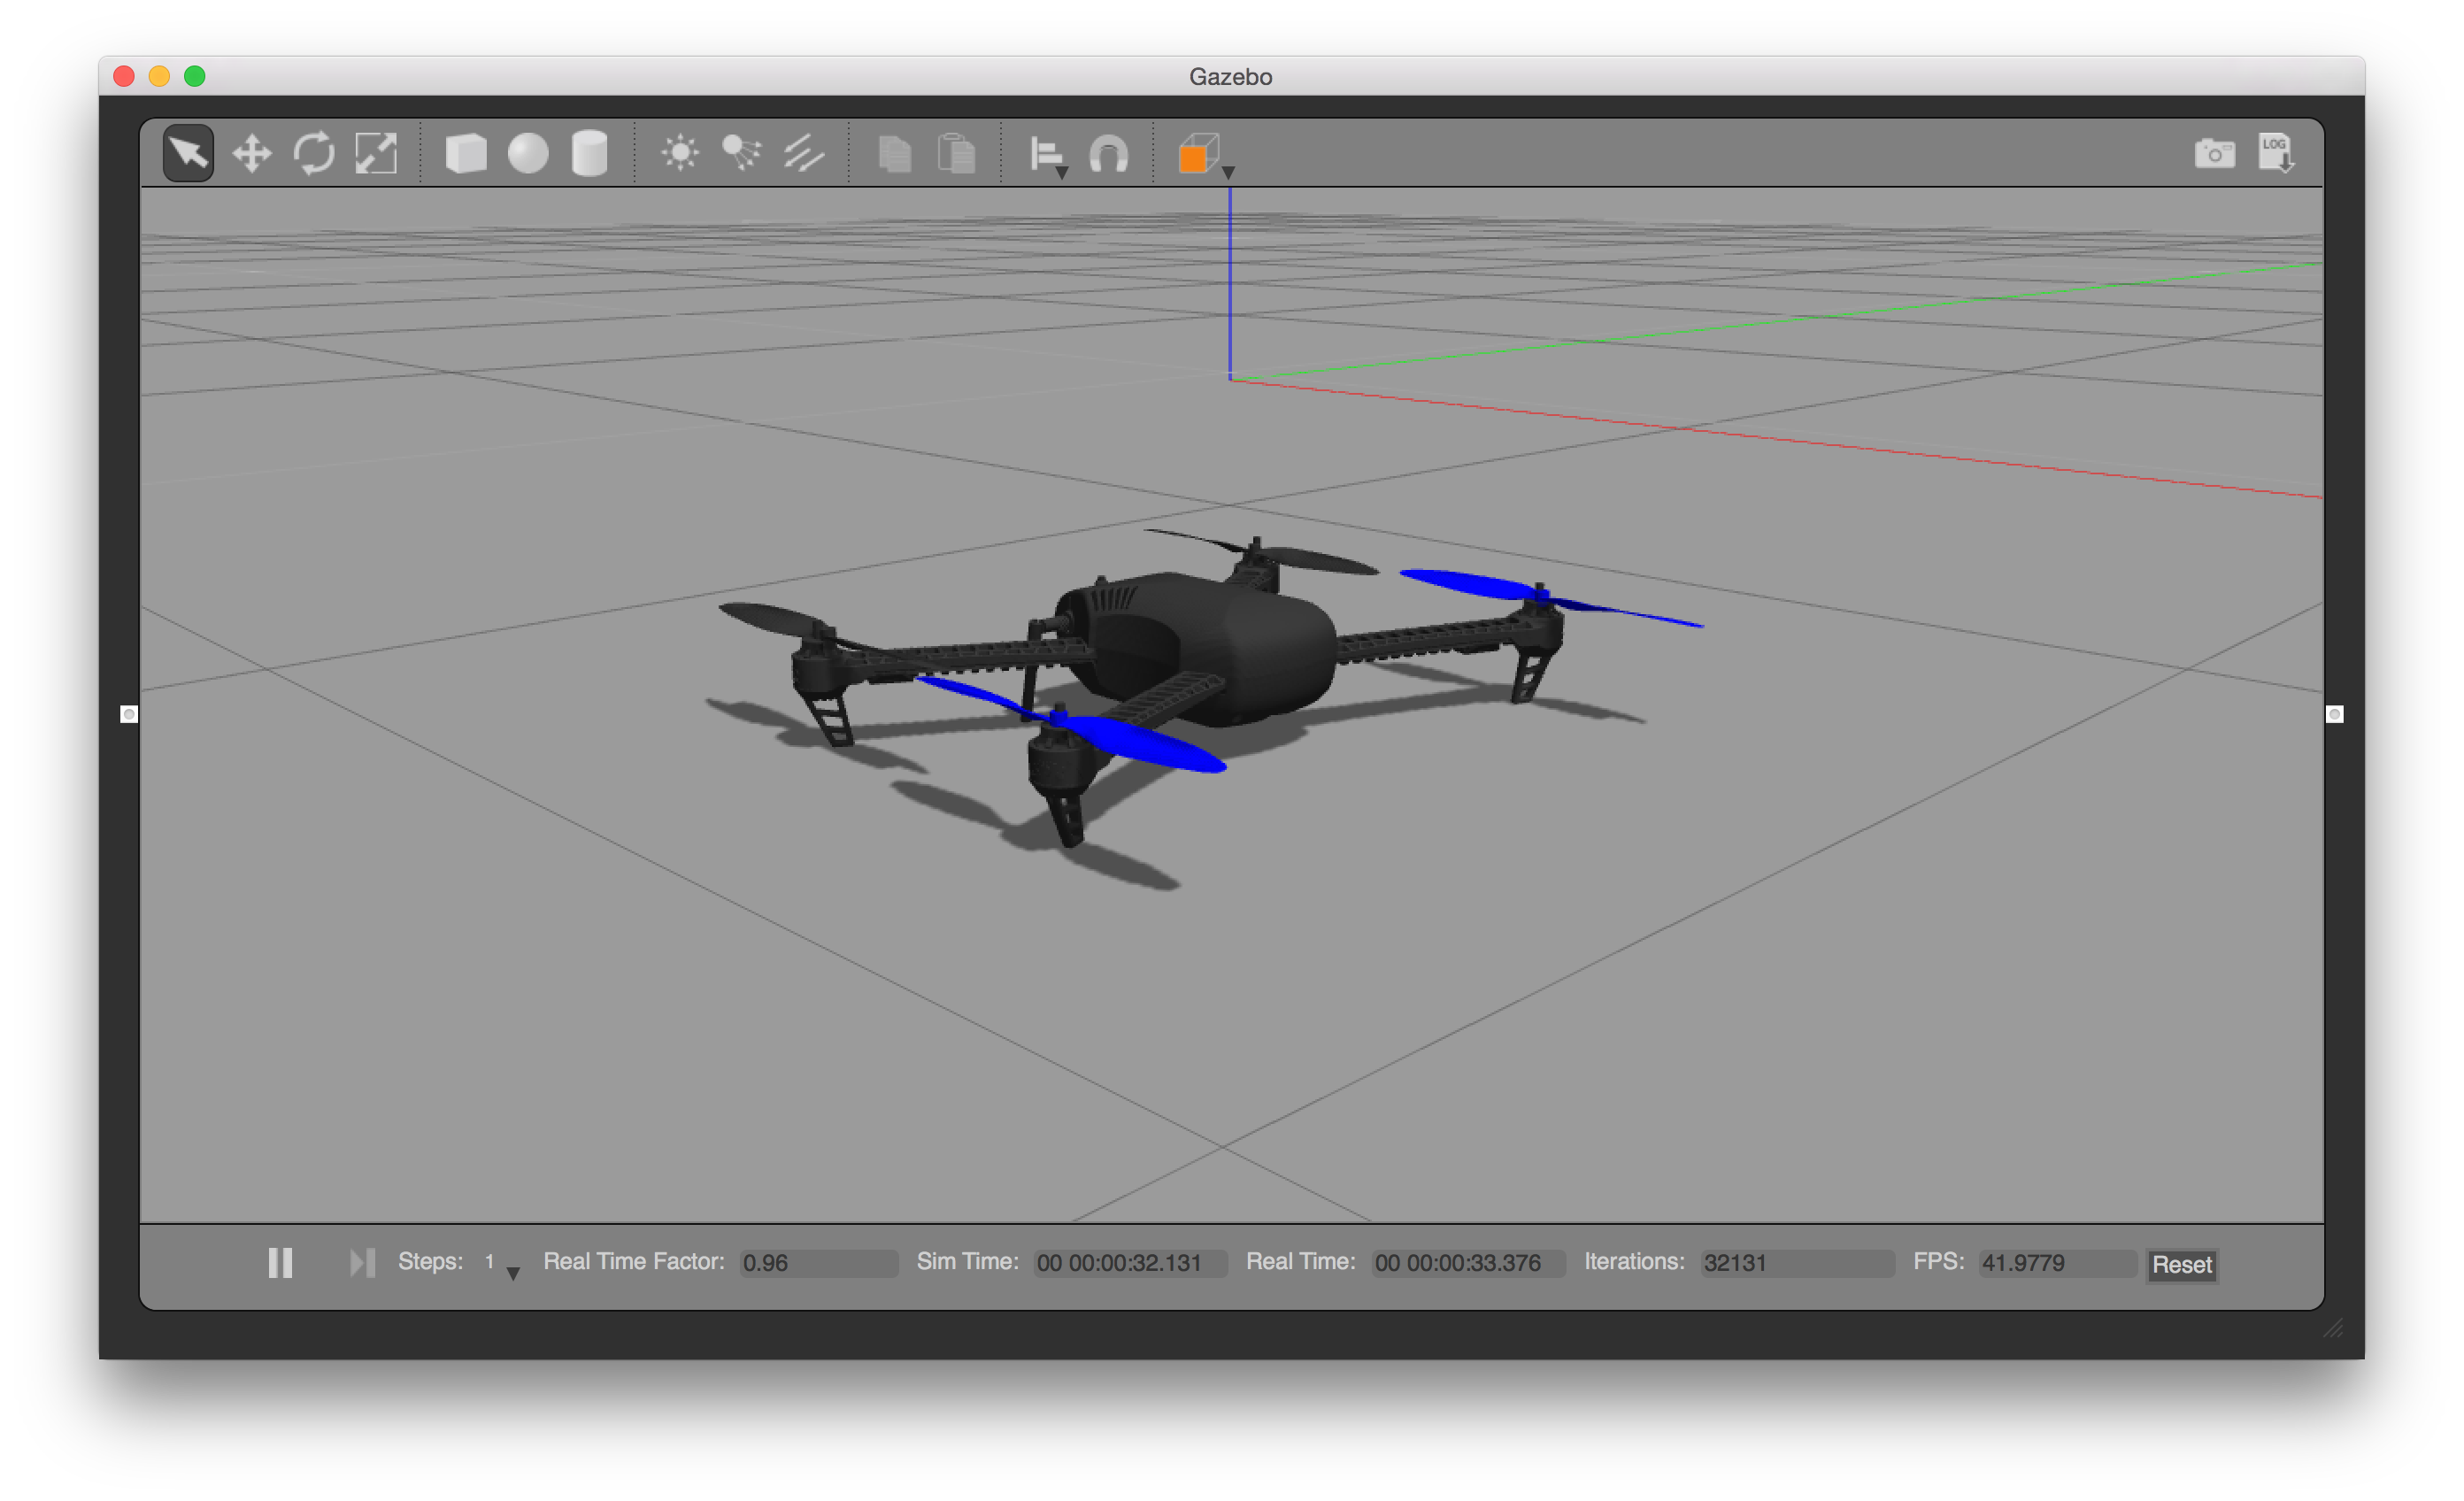
\includegraphics[width=140mm]{figures/iris_gazebo.png}
    \caption{PX4 Simulation using Gazebo with ROS wrapper}
    \label{fig:px4_sitl_ros_wrapper}
\end{figure}

\section{QGroundControl}
TODO QGroundControl description
